\chapter{XIBO-Grundlagen}
\section{Digital Signage}\label{sec:digitalsignage}
Digital Signage Systeme haben die Aufgabe viele Bildschirme mit Inhalten zu füllen und eventuell auch diese Inhalte zu designen. Damit soll das zeit- oder interaktionsgesteuerte ändern von Inhalten auf den Bildschirmen einfach und unübersichtlich gehalten werden. Digital Signage bietet ein breites Spektrum an Anwendungsbereichen.    https://de.wikipedia.org/wiki/Digital_Signage#Anwendungsbeispiele:_2017.

\section{Was ist XIBO?}\label{sec:xibo}
Das XIBO ist ein Open Source Digital Signage System entwickelt von der Spring Signage LTD. Das XIBO-System besteht aus vielen verschiedenen Komponenten. Das XIBO Paket besteht aus einem klassischen Server-Client Konstrukt. Der Server besteht aus 3 Komponenten Content Managment System das mithilfe von ZeroMq bei Anderung der Inhalte diese aktualisieren soll, einer Datenbank und einer Weboberfläche die es dem Benutzer ermöglichen soll das System zu bedienen.

SYSTEM ARCH PLAN eventuell noch über zeromq schreiben

\section{Weboberfläche des XIBO}\label{sec:webpagexibo}
Das Steuerungszentrum des ganzen Signage System ist die Weboberfläche die ganz einfach über einen Browser unter der Serveraddresse aufgerufen werden kann. Auf der Willkommenseite sind die wichtigsten Funktionen dargestellt:

\begin{enumerate}
	\item {\em Kalender:} Mit der Kalender Funktion kann eingetragen werden zu welchen Zeitpunkt welcher Inhalt auf welchem Bildschirm angezeigt werden soll. In dem Xibo-Kalender werden auch bereits eingetragene Aktivitäten angezeigt.

\begin{calendar}
	\centering
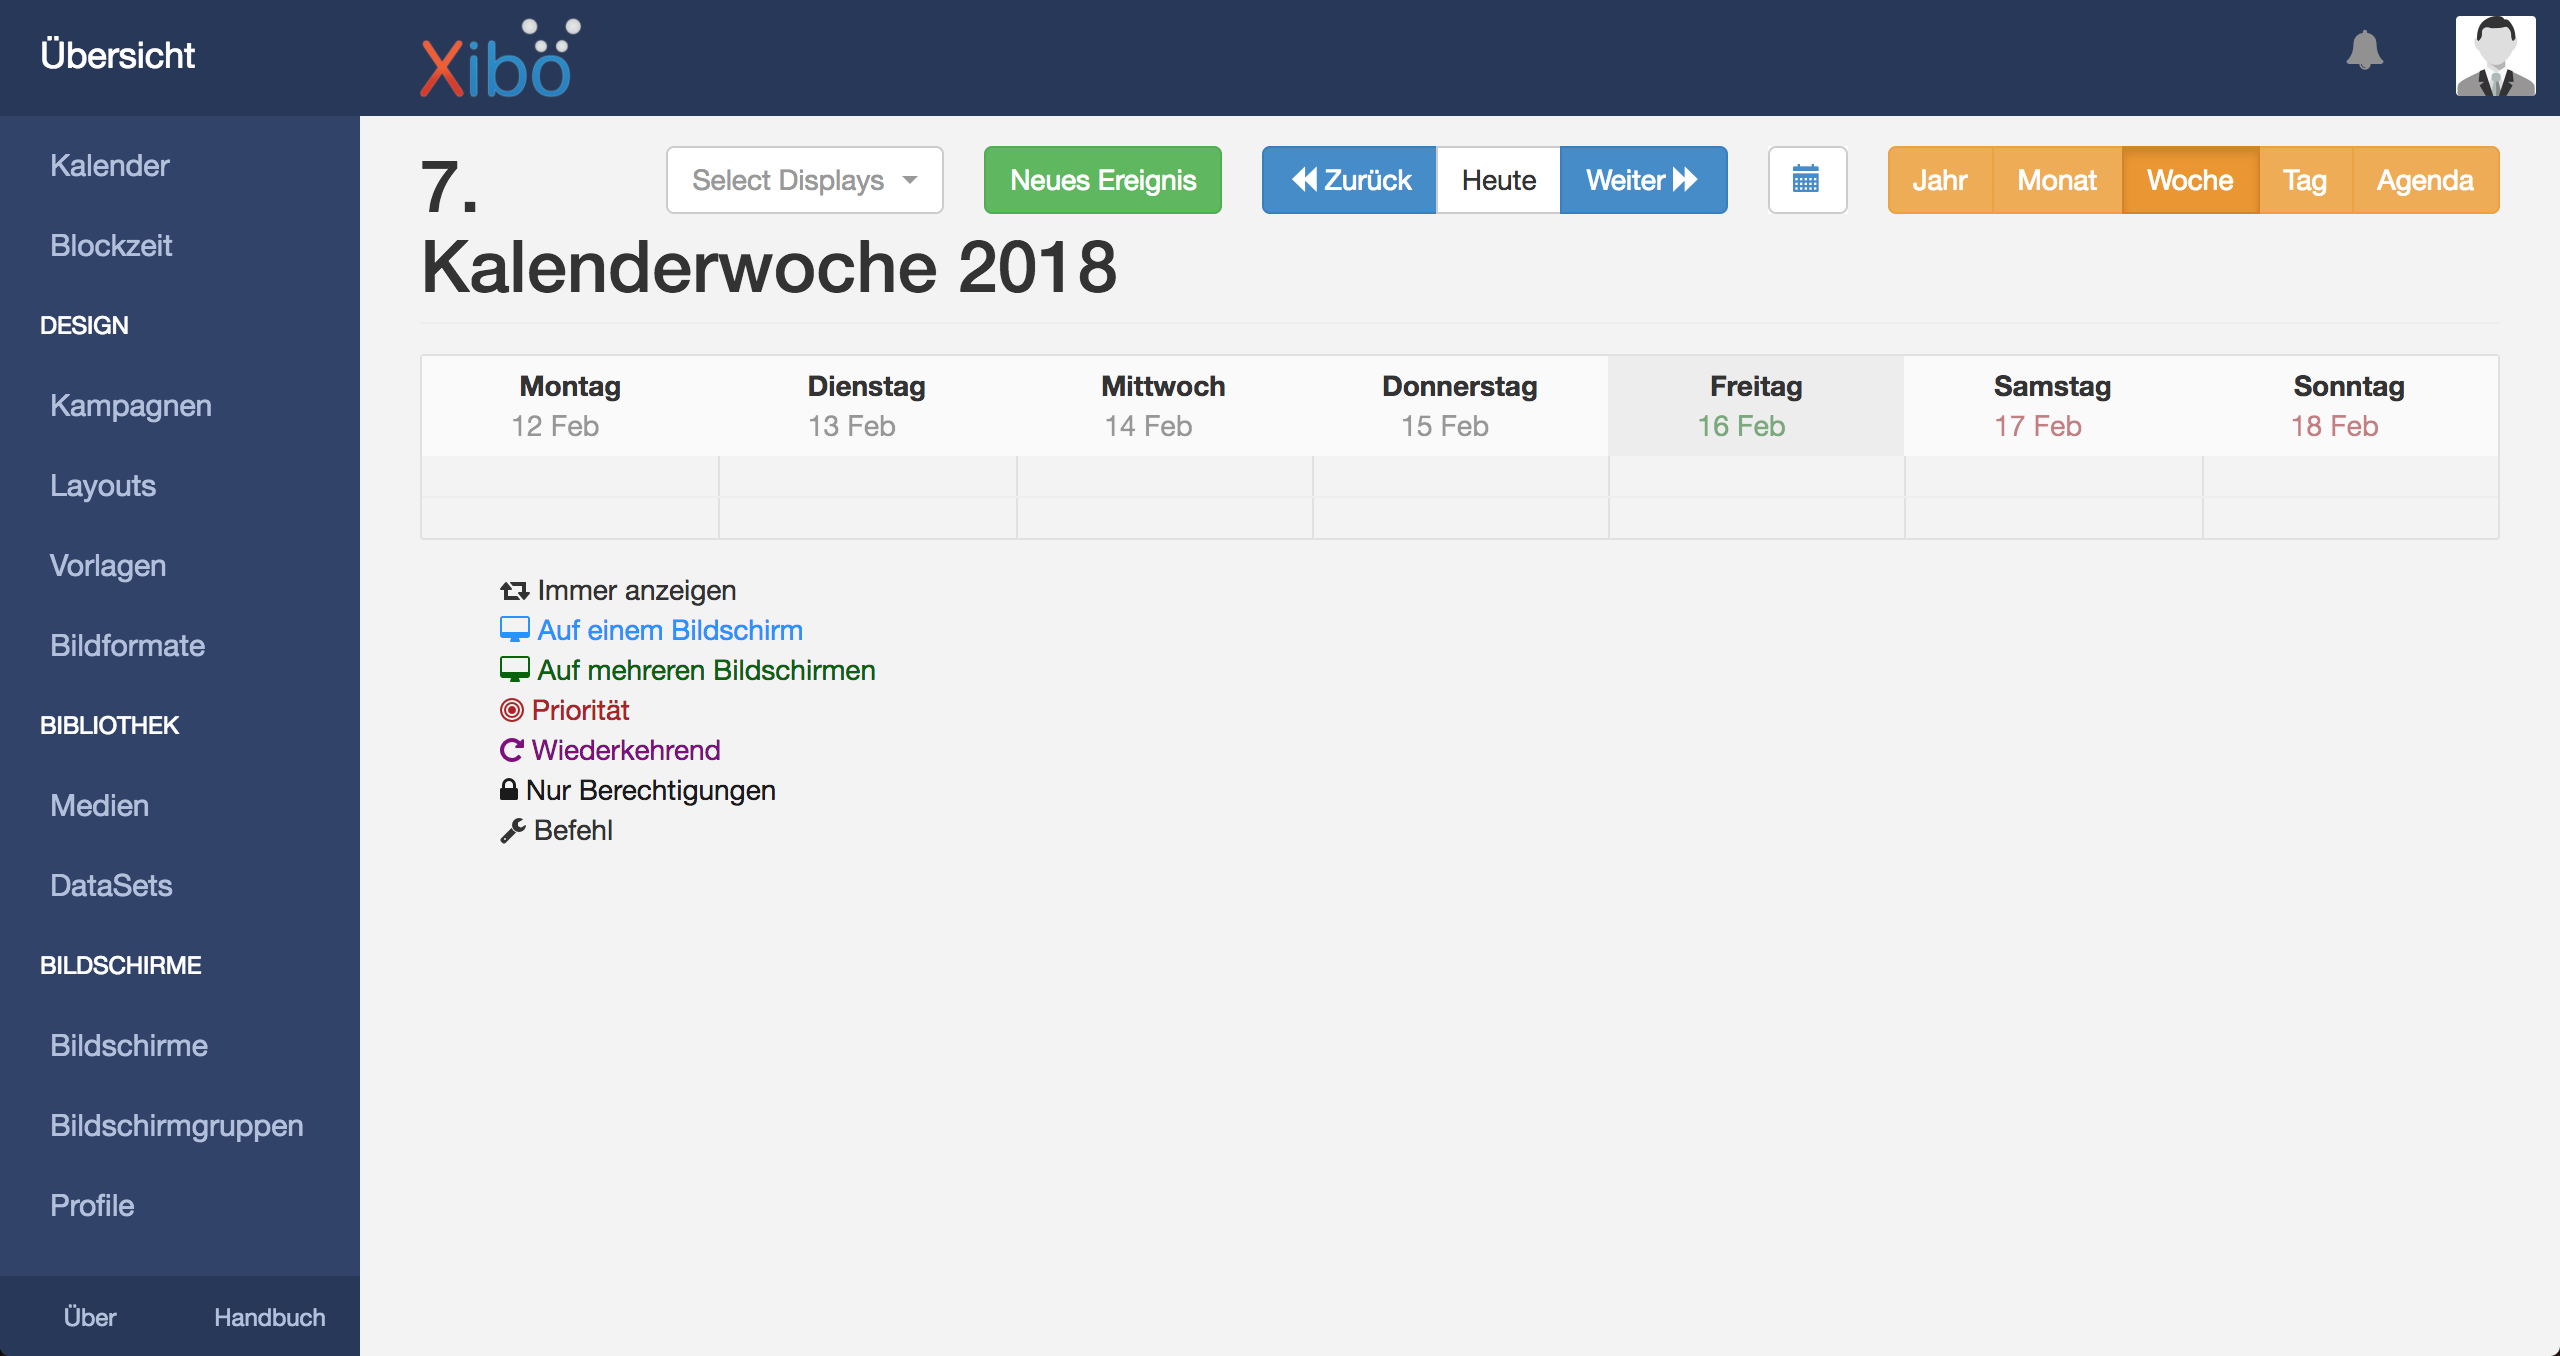
\includegraphics[width=1\textwidth]{images/xibo-basics-calendar}
	\label{Calendar}
\end{calendar}	
	
	\item {\em Layouts:} 
	Die Layout Funktion ist einer der wichtigsten Komponenten des Signage Systems es beschäftigt sich mit dem designen der Inhalte. Auf diese Funktion kommen wir noch einmal zurück
	
	\item {\em Bibliothek:} 
	Die Bibliothek Funktion ist zuständig für das Verwalten der Medien. Hier können Sie verschiedene Dateien hochladen.  Diese Medien können dann in Layouts eingebunden und angezeigt werden.
	
	\item {\em Benutzer:} 
	Im Menüpunkt Benutzer können neue Benutzer angelegt werden und bereits bestehende bearbeitet oder gelöscht werden. Dabei gibt es auch ein Rechte-System. Es könnne auch Datenmengen Begrenzungen pro Benutzer eingestellt werden.
	
	\item {\em Einstellungen:} 
	Der Menüpunkt Einstellung gibt dem Nutzer die Möglichkeit verschiedene Optionen einzustellen. So sind zum Beispiel die richtige Zeitzone, E-Mail Benachrichtigungen wichtige Einstellungen die für ein Einwandfreies funktionieren des Xibo-Servers zuständig wichtig sind.
\end{enumerate}

\section{Designen mit XIBO}\label{sec:designexibo}
Beim Designen von einem neuen Layout im XIBO muss zuerst die Bildschirm auflösung ausgewählt werden. Und dem Layout ein passender Name zugewiesen werden sowie optional auch eine Beschreibung. 

\textbf{Layout Maske}

\begin{calendar}
	\centering
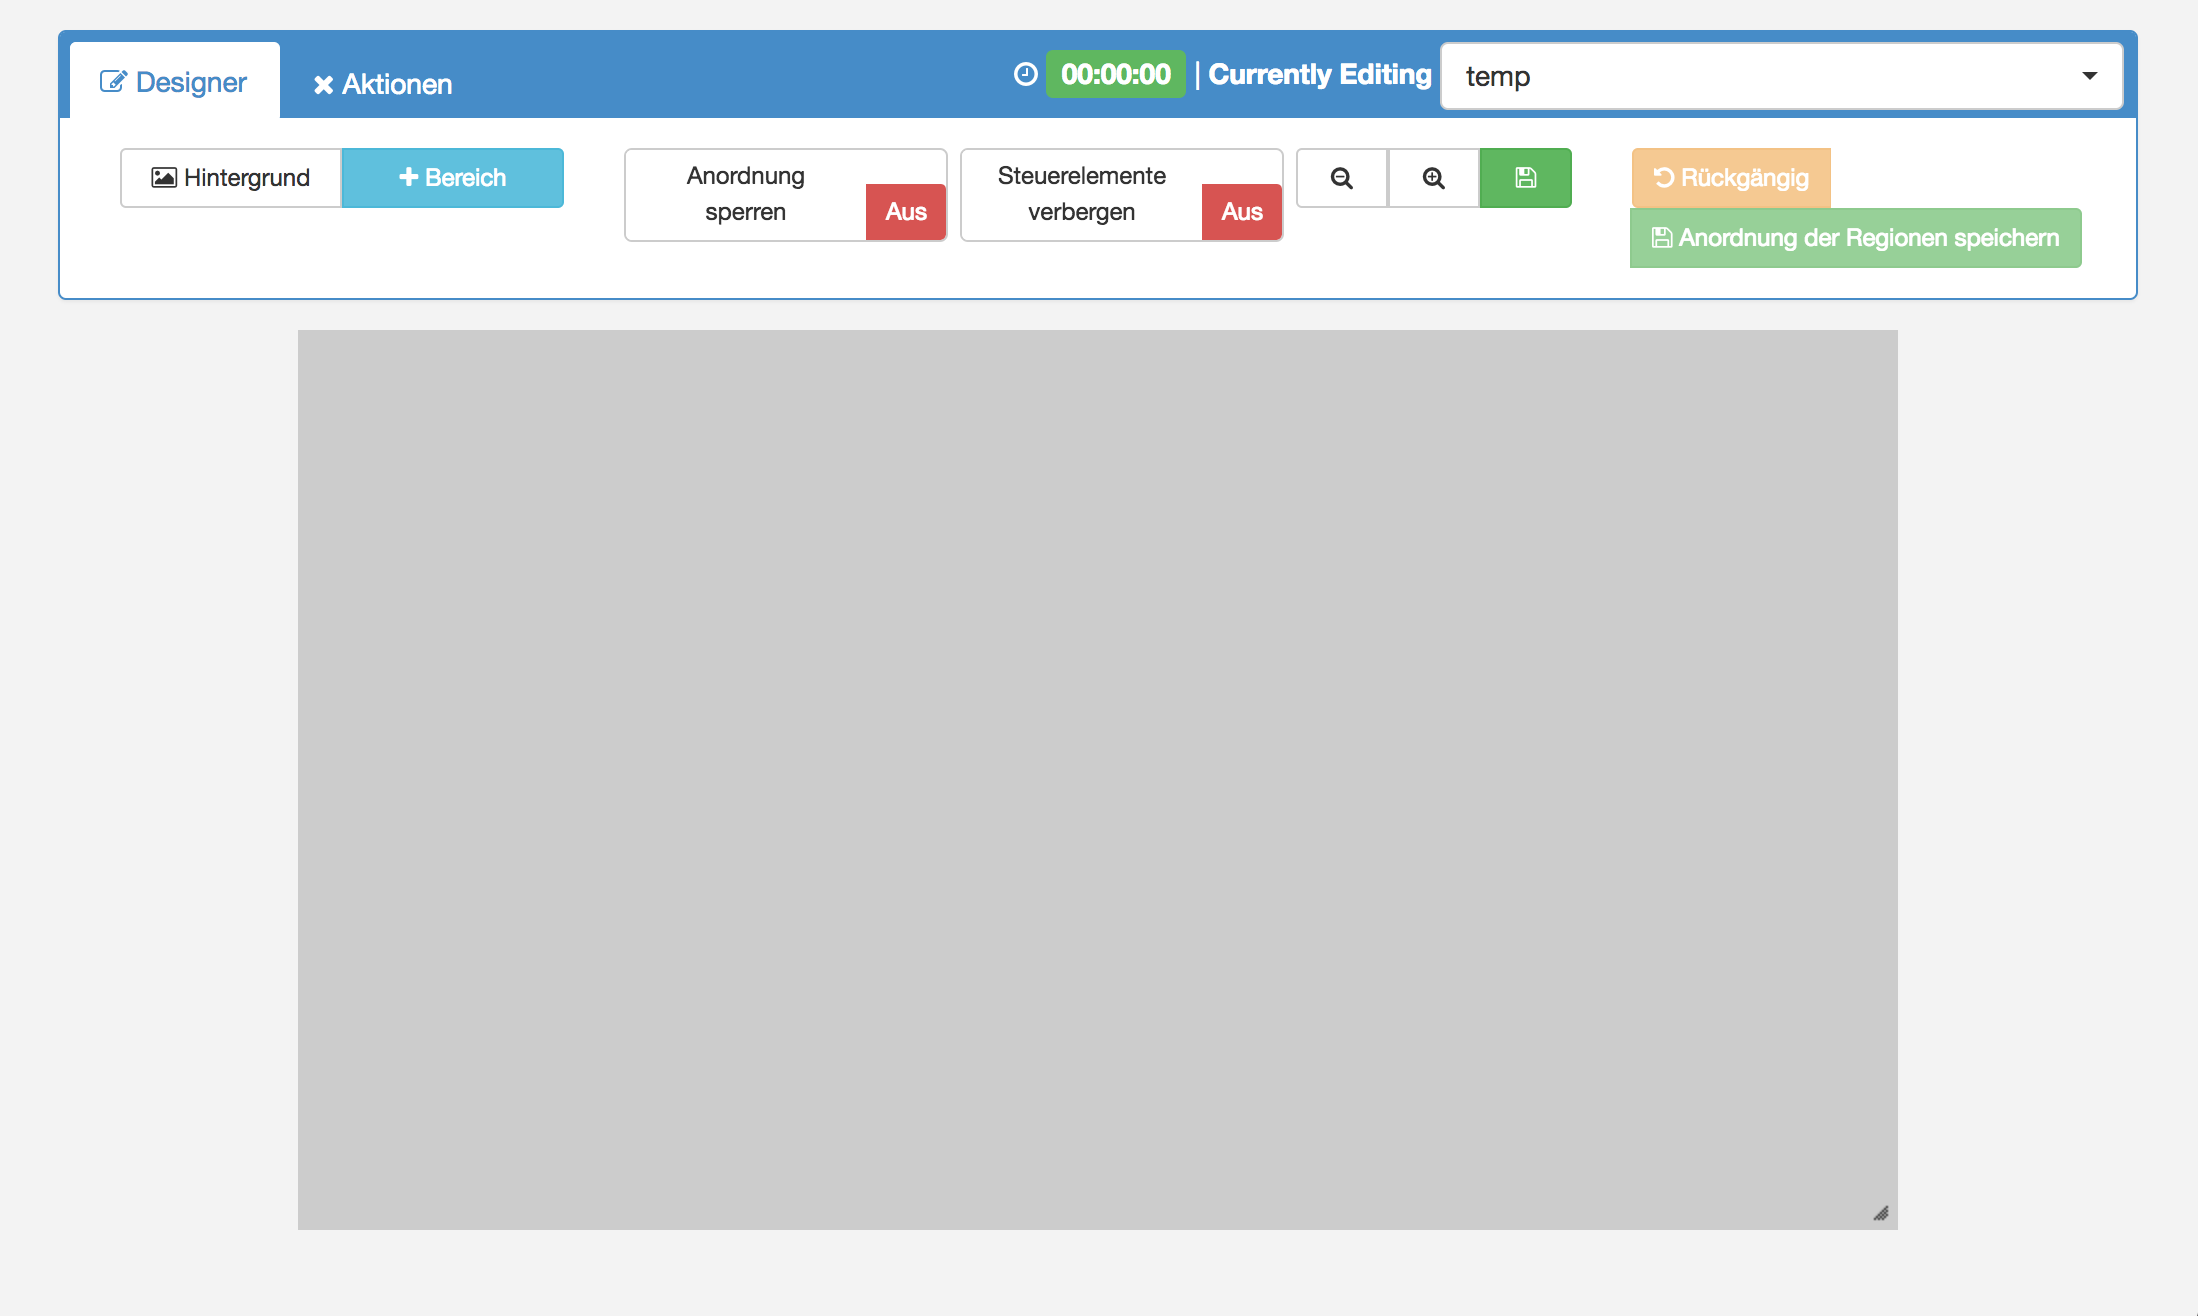
\includegraphics[width=1\textwidth]{images/xibo-basics-designer}
	\label{Calendar}
\end{calendar}	

Dem Layout kann nun eine Region oder auch mehrere  hinzugefügt werden eine Region kann wiederrum mehrere Widgets enthalten. Mit einem Doppelklick auf die Region kann ein Widget hinzugefügt werden. Es gibt viele verschiedene Arten von Widgets:

\begin{widgettypes}
	\item {\em Bibliothek:} Mit diesem Widget können Dateien aus der Medienbibliothek in die Region angezeigt werden. 

	
	\item {\em Uhr:} 
	Dieser Widgettyp bindet eine Uhr in die aus
	
	\item {\em Bibliothek:} 
	Die Bibliothek Funktion ist zuständig für das Verwalten der Medien. Hier können Sie verschiedene Dateien hochladen.  Diese Medien können dann in Layouts eingebunden und angezeigt werden.
	
	\item {\em Benutzer:} 
	Im Menüpunkt Benutzer können neue Benutzer angelegt werden und bereits bestehende bearbeitet oder gelöscht werden. Dabei gibt es auch ein Rechte-System. Es könnne auch Datenmengen Begrenzungen pro Benutzer eingestellt werden.
	
	\item {\em Einstellungen:} 
	Der Menüpunkt Einstellung gibt dem Nutzer die Möglichkeit verschiedene Optionen einzustellen. So sind zum Beispiel die richtige Zeitzone, E-Mail Benachrichtigungen wichtige Einstellungen die für ein Einwandfreies funktionieren des Xibo-Servers zuständig wichtig sind.
\end{widgettypes}

